
$a$: amplitude\\
$\rG$: \textit{Gaussian radius} \ie twice Gaussian \textit{std} \\
$H$: Gaussian amplitude\\
$A$: determined area\\
$r$: determined radius\\
with $A=\pi r^2$ and $V=2\pi\sigma^2$
\begin{align}
 H-a 
&= 
H \exp \left( -\frac{A}{2 \pi \left( \rG/2 \right)^2}  \right) \\ 
\end{align}
and

\begin{align}
 H-a 
&= 
H \exp \left( -\frac{A}{2 \pi \left( \rG/2 \right)^2}  \right) \\
  1-a/H 
&= 
 \exp \left( -\frac{2A}{\pi \rG^2}  \right) \\
  \pi \rG^2
&= 
  \left( -\frac{2A}{\ln \l 1-a/H \r }  \right) \\
 \rG
&= 
 \sqrt{-\frac{2A}{\pi \ln \l 1-a/H \r }}  \\
\end{align}
















with $\gamma=-\frac{1}{2 \sigma^2} $ \\
\begin{align}
g(x,y)= h \exp \left(\gamma \left(  y^2 + x^2 \right) \right)
\end{align}

\begin{align}
V =  \int_{-r}^{r}\int_{-r}^{r} g \dint{x}\dint{y}
\end{align}

\begin{align}
	\lambda(r) &= \frac{V}{A^{1.5}}\\
		&= 
	\frac{  \int_{-r}^{r}\int_{-r}^{r} g \dint{x}\dint{y}}
{ \left(   \pi r^2  \right)^{3/2}}\\
&=
 \left(r \sqrt{\pi}    \right)^{-3}
 \int_{-r}^{r}\int_{-r}^{r} g \dint{x}\dint{y}\\
&=
   \left(r \sqrt{\pi}    \right)^{-3}
\int_{-r}^{r} \left[   \frac{  g }{ 2\gamma x} \right]^{r}_{-r} \dint{y}\\
&=
 \left(r \sqrt{\pi}    \right)^{-3}
\int_{-r}^{r} 
 \frac{  \exp \left(\gamma \left(  y^2 + r^2 \right) \right)   }{ 2 \gamma r}
-  \frac{  \exp \left(\gamma \left(  y^2 + r^2 \right) \right)   }{- 2 \gamma r}
  \dint{y}\\
&=
 \left(r \sqrt{\pi}    \right)^{-3}
\int_{-r}^{r} 
 \exp \left(\gamma \left(  y^2 + r^2 \right) \right) 
\left( 
 \frac{  1 }{  \gamma r}
 \right)
  \dint{y}\\
&=
\left( \gamma r^4 \pi^{3/2}  \right)^{-1}
\int_{-r}^{r} g(r,y) \dint{y}\\
&=
\left( \gamma r^4 \pi^{3/2}  \right)^{-1}
\int_{-r}^{r} g(r,y) \dint{y}\\
&=
h\left( \gamma r^4 \pi^{3/2}  \right)^{-1}
 \frac{  \exp \left(\gamma \left(  y^2 + r^2 \right) \right)  }{ \gamma r}  \\
&=
h\left( \gamma^2 r^5 \pi^{3/2}  \right)^{-1}
 g(r,r)   \\
&=
h^2 \pi^{2/3}
\frac
{
\exp \left(\gamma \left(  2 r^2 \right) \right)
}
{
\gamma^2 r^5 
}
\end{align}

\begin{align}
&= 
\frac
{
\exp \left( 2 r^2  \right)
}
{
r^5 
}
\end{align}
% 
% 
% $A_{\circ}$ : area of circle with equal perimeter
% %%....................................................................
% \begin{align}
% 	q_a
% 	&=
% 	\frac{A}{A_{\circ}}  \\
% 	&=
% 	\frac{A}{   \pi r_{\circ}^2   }  \\
% 	&=
% 	 \frac{A}{   \pi \left( \frac{p}{2 \pi} \right)^2   }  \\
% 	&=
% 	4 \pi\frac{A}{   p^2   }  
% \end{align}
% %%....................................................................
% $p_{\circ}$ : perimeter of circle with equal area
% %%....................................................................
% \begin{align}
% 	q_s
% 	&=
% 	\frac{p_{\circ}}{p}  \\
% 	&=
% 	\frac{ 2 \pi r_{\circ} }{p}  \\
% 	&=
% 	\frac{ 2 \pi \sqrt{ A/\pi  }}{p}  \\
%  	&=
% 	\frac{ 2  \sqrt{\pi A }}{p} \\
% &=
% \sqrt{q_a}
% \end{align}
% %%....................................................................
% 
% 
% 
% \begin{figure}[!ht]
% 	\centering
% 	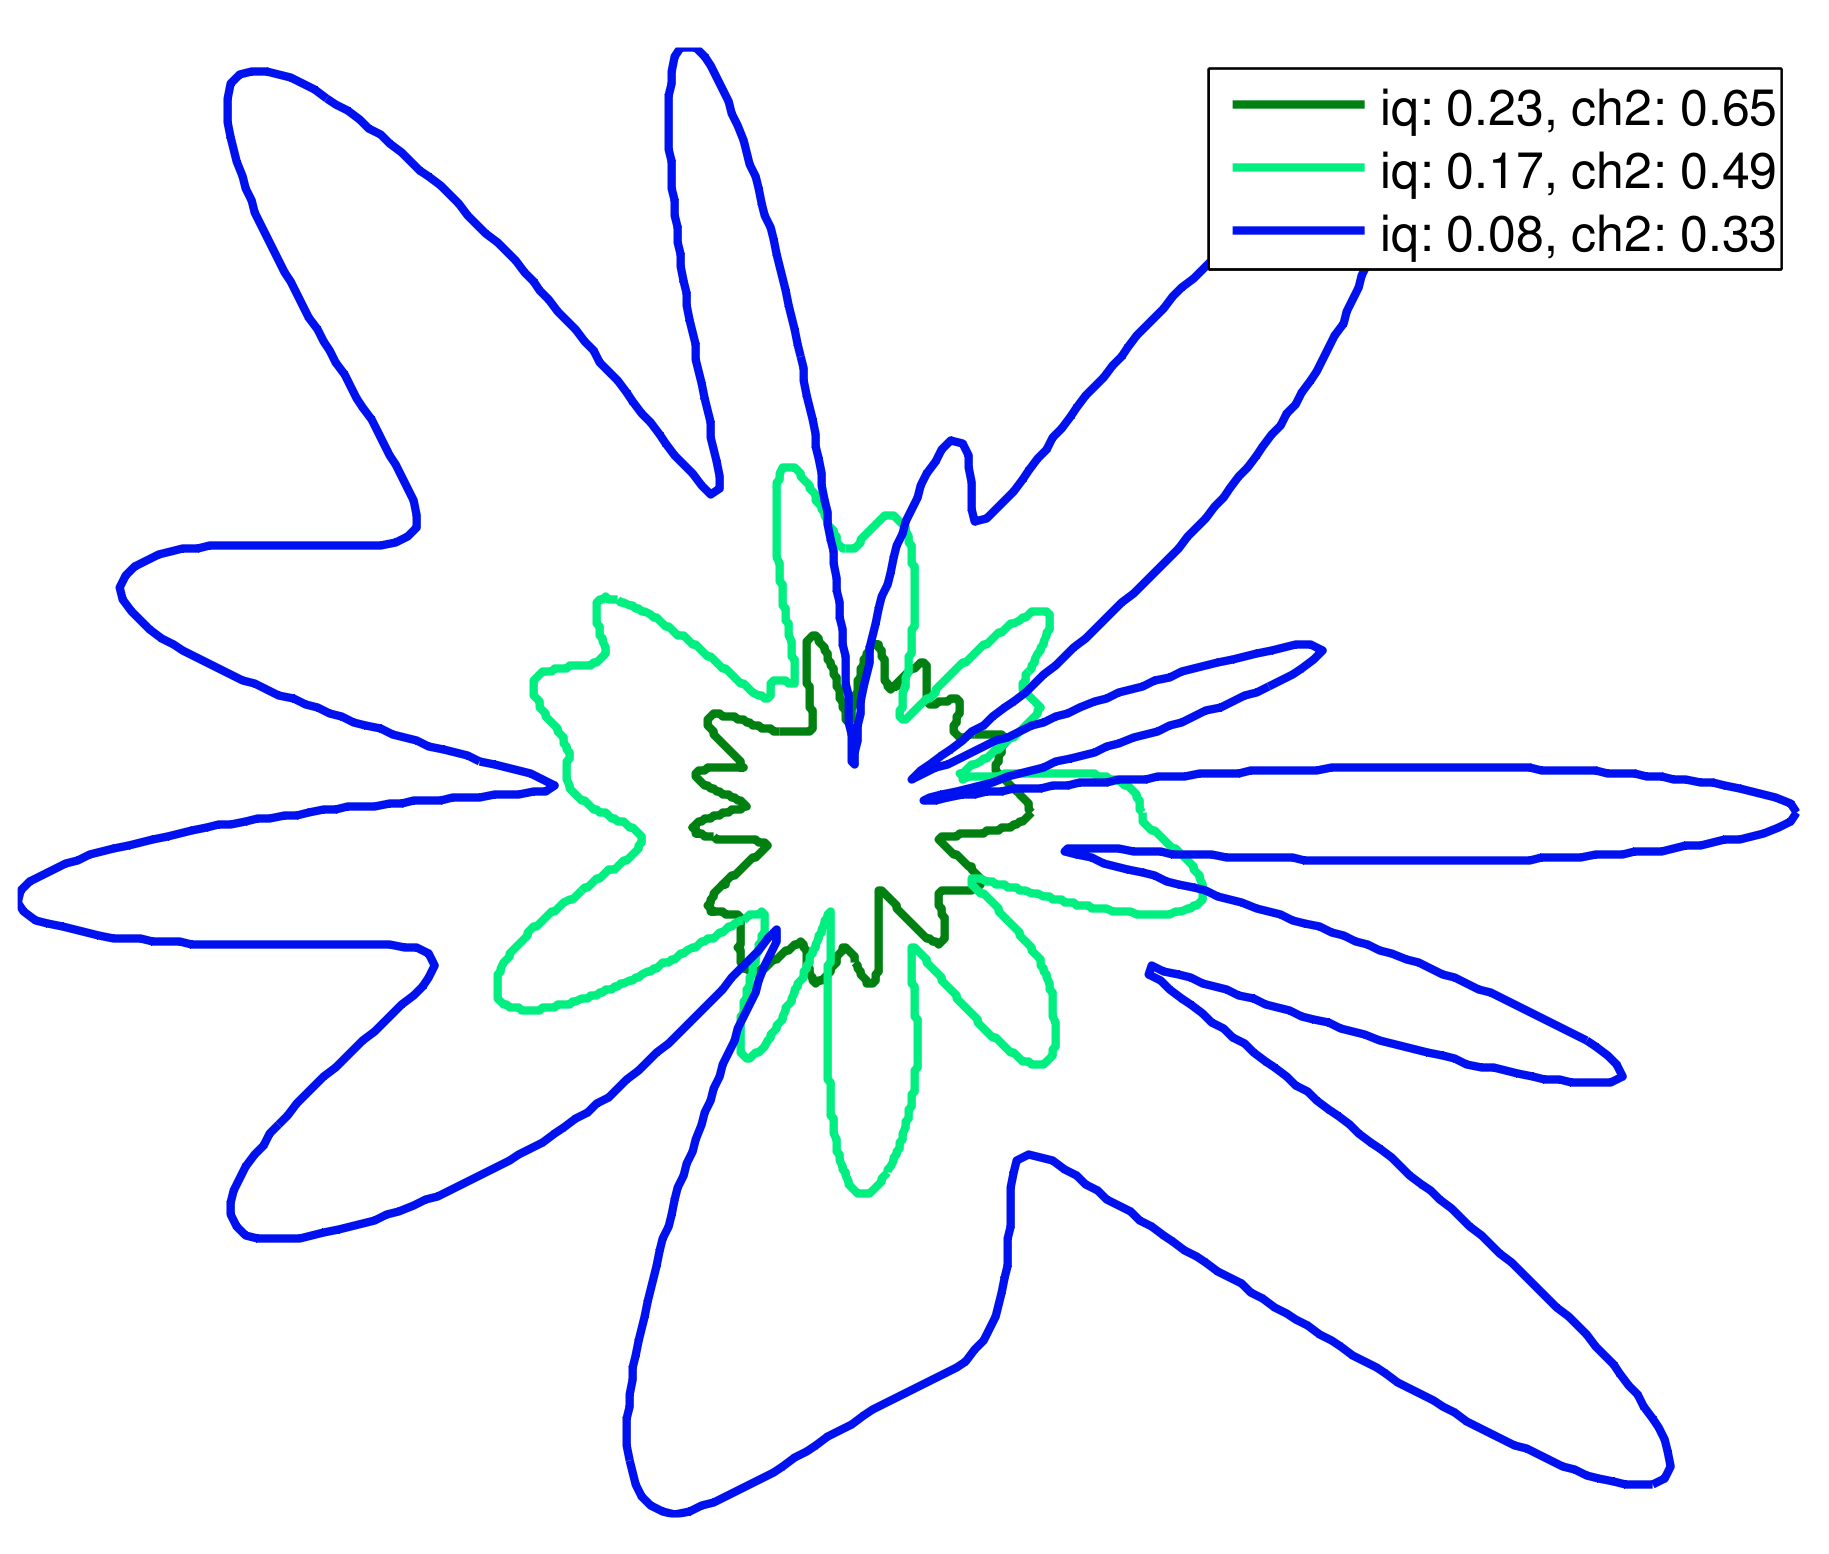
\includegraphics[scale=.7]{./huh.png}
% 	% huh.png: 1829x1554 pixel, 300dpi, 15.49x13.16 cm, bb=0 0 439 373
% \end{figure}
% 
% 
% 
% chelton:
% %%....................................................................
% \begin{align}
% h_a
% &=
% \frac{d}{\mu}
% \end{align}
% with
% \begin{equation}
% \mu=
% \begin{cases}
% 	400km &; \norm{\phi} > 25^{\circ}  \\
% 	\left( 800 \frac{\left( 25-\norm{\phi}  \right)}{25} + 400  \right) km &; \norm{\phi} \leqslant 25^{\circ}
% \end{cases}
% \end{equation}
% %%....................................................................
% alternative
% %%....................................................................
% \begin{align}
% h_b
% &=
% 4 \pi \frac{A}{ \left( \pi d  \right)^2}  \\
% &=
% 4 \frac{A}{ \pi d^2}  
% \end{align}
% %%....................................................................
% 
% 
% 



Integrating \eqref{eq:Emech1} over a closed Volume with standard boundary conditions yields a Eularian equation
for the change in total mechanical energy of the domain (Note that the advection term does just that - \textit{advect}.
It has no contribution to the total change of energy).
%%....................................................................
\begin{equation}\begin{split}
\frac{1}{2}\left(
	\int_{V} \frac{\partial \vec{u}^2}{\partial t}  \; \mathrm{d}V
  +
	\int_{V} \vec{u} \cdot \grad \vec{u}^2 \; \mathrm{d}V
	\right)
	&=
	\int_{V} \vec{u}\cdot \nu  \vec{\nabla}^{2} \vec{u}  \; \mathrm{d}V \\
	%%--------------------------------------------------------------------
	\int_{V} \frac{\partial \Em}{\partial t}  \; \mathrm{d}V
	&=
	\int_{V} \nu\left(
	\frac{1}{2}\grad^2 \vec{u}^2 - \norm{\grad \vec{u}}^2
	\right)  \; \mathrm{d}V
\end{split}\end{equation}
%%....................................................................


%%####################################################################
%%####################################################################


%%####################################################################
%%####################################################################


\section{2D-Turbulence}
oiug
\subsection{Aspect Ratio}
\subsection{Enstrophy Conservation}
Without a third dimension, vorticity can no longer be altered by stretching or tilting.
\eqref{eq:vort2} then reduces to:
\begin{equation}\begin{split}
	\frac{D \omega_{a}}{D t}
	&=
	\nu \grad^{2} \omega
\end{split}\end{equation}
In other words, in absence of friction, besides energy, now also vorticity is materially conserved.
\subsubsection{}


\begin{equation}\begin{split}
	\int_A \omega \frac{D \omega_{a}}{D t}\; \mathrm{d}A
	&=
	\nu\int_A  \omega \grad^{2} \omega\; \mathrm{d}A\\
	\frac{\partial \Enstro}{\partial t}
	=
	\frac{\partial }{2\partial t} \int_A \omega^2 \; \mathrm{d}A
	&=
	\nu\int_A \frac{1}{2}\grad^{2} \omega^{2} - \norm{\grad \omega}^2  \; \mathrm{d}A \\
	&=
	\frac{\nu}{2}\oint_A \grad \omega^{2} \cdot \mathrm{d}\vec{s}
	- \int_A\norm{\grad \omega}^2  \; \mathrm{d}A \label{eq:enst1}	\\
\end{split}\end{equation}


\begin{equation}\begin{split}
	\int_A \omega \frac{D \omega_{a}}{D t}\; \mathrm{d}A
	&=
	\nu\int_A  \omega \grad^{2} \omega\; \mathrm{d}A\\
	\frac{\partial \Enstro}{\partial t}
	=
	\frac{\partial }{2\partial t} \int_A \omega^2 \; \mathrm{d}A
	&=
	\nu\int_A \omega  \frac{\partial }{\partial x_i} \vec{e}_i \frac{\partial  \omega}{\partial x_i} \vec{e}_i\; \mathrm{d}A \\
	&=
	\nu\int_A \omega  \frac{\partial^2  \omega}{\partial x_i^2} \; \mathrm{d}A \\
	%%--------------------------------------------------------------------
	&=
	\nu\int_A \frac{1}{2} \frac{\partial^2 \omega^2 }{\partial x_i^2}  - \left(\frac{\partial  \omega}{\partial x_i} \right)^2 \; \mathrm{d}A \label{eq:enst1}
\end{split}\end{equation}
If we now consider an infinite domain with fading $\vec{u}$ away from the center,
the first RHS-term of \eqref{eq:enst1} vanishes, leaving:
\begin{equation}\begin{split}
	\frac{\partial \Enstro}{\partial t}
	&=
	- \int_A \nu\left(\frac{\partial  \omega}{\partial x_i} \right)^2 \; \mathrm{d}A \\
	&=
	- \int_A \nu\norm{ \grad \omega}^2 \; \mathrm{d}A
\end{split}\end{equation}



In 2 dimensions enstrophy can also be rewritten as follows:
%%....................................................................
\begin{equation}\begin{split}
\Enstro
&=
\int_{V} \norm{\vec{\omega}}^{2}  \; \mathrm{d}V\\
&=
\int_{V} \omega^{2}  \; \mathrm{d}V\\
&=
\int_{V} \left( \frac{\partial v}{\partial x} - \frac{\partial u}{\partial y} \right)^2  \; \mathrm{d}V\\
&=
\int_{V} \left(\frac{\partial v}{\partial x}\right)^2
-2\frac{\partial v}{\partial x} \frac{\partial u}{\partial y}
+ \left(\frac{\partial u}{\partial y} \right)^2  \; \mathrm{d}V\\
&=
\int_{V} \left(\frac{\partial v}{\partial x}\right)^2
+ \left(\frac{\partial u}{\partial y} \right)^2
-2\frac{\partial v}{\partial x} \frac{\partial u}{\partial y}
+ \left( \div \vec{u} \right)^2
  \; \mathrm{d}V\\
&=
\int_{V} \left(\frac{\partial v}{\partial x}\right)^2
+ \left(\frac{\partial u}{\partial y} \right)^2
+\left(\frac{\partial v}{\partial y}\right)^2
+ \left(\frac{\partial u}{\partial x} \right)^2
  \; \mathrm{d}V\\
  &=
\int_{V}
\norm{\grad \vec{u}}^2
\; \mathrm{d}V\\
  &=
\int_{V}
\frac{1}{2} \grad^2 \vec{u}^2 -\vec{u} \cdot \grad^2 \vec{u}
\; \mathrm{d}V\\
  &=
\frac{1}{2}\oint_{A}   \grad \vec{u}^2 \cdot  \; \mathrm{d}\vec{s}
-\int_{V}\vec{u} \cdot \grad^2 \vec{u}  \; \mathrm{d}V\\
  &=
\int_{V}
-\vec{u} \cdot \grad^2 \vec{u}
\; \mathrm{d}V\\
\end{split}\end{equation}
\textit{...under appropriate boundary conditions} WHY???\\
%%--------------------------------------------------------------------
combinging ... and ... reveals the coupling	that energy dissipation is proportional to the total enstrophy of the system.
And that


\begin{equation}\begin{split}
	\int_{V}\frac{\partial E_{m}}{\partial t} \; \mathrm{d}V
	&=
	-\nu \int_{V} \norm{\vec{\omega}}^{2}  \; \mathrm{d}V \\
	%%--------------------------------------------------------------------
	&=
	-\nu \Enstro\\
	\int_{V}\frac{\partial E_{m}}{\partial t} \; \mathrm{d}V
	&=
	\grad^{2} \frac{D \Enstro}{D t}
\end{split}\end{equation}



\chapter{junk}



%%....................................................................
\begin{equation}\begin{split}
	\frac{\partial \enstro}{\partial t}
	+
	\vec{u} \cdot \grad \enstro
	&=
	-\nu \grad^{2} \enstro\\
	\frac{\partial \norm{\grad \vec{u}}^{2}}{\partial t}
	+
	\vec{u} \cdot \grad \norm{\grad \vec{u}}^{2}
	&=
	-\nu \grad^{2} \norm{\grad \vec{u}}^{2}\\
	\frac{\partial }{\partial t} \left(\frac{\partial u_{i}}{\partial x_{j}}\right)^{2}
	+
	u_{k}  \frac{\partial}{\partial x_{k}} \left(\frac{\partial u_{i}}{\partial x_{j}}\right)^{2}
	&=
	-\nu \grad^{2}  \left(\frac{\partial u_{i}}{\partial x_{j}}\right)^{2}\\
\end{split}\end{equation}


\begin{equation}\begin{split}
	\frac{\partial \enstro}{\partial t}
&=
	-
	\vec{u} \cdot \grad \enstro
	-\nu \grad^{2} \enstro{}
	+\vec{\omega}_{a}\cdot \left( \vec{\vec{\omega}_{a}} \cdot \grad \right) \vec{\vec{u}}\\
&\sim-
	\frac{U^{3}}{L^{3}}
	- \frac{\nu U^{2}}{L^{4}}
	+ \frac{U^{3}}{L^{3}}\\
\end{split}\end{equation}

\begin{equation}\begin{split}
	\frac{\partial E_{m}}{\partial t}
&\sim{}
-	\frac{U^{3}}{L}
	- \frac{\nu U^{2}}{L^{2}} \\
	&\sim
	\frac{\partial \enstro}{\partial t} L^{2}
\end{split}\end{equation}






